\documentclass{ctexart}

\usepackage{van-de-la-sehen}

\begin{document}

\renewcommand{\arraystretch}{1.5}

\section{特殊构型, 唯一性定理, 电像法与Green定理等} % (fold)
\label{sec:特殊构型_唯一性定理_电像法与green定理等}

\subsection{本构关系} % (fold)
\label{sub:本构关系}

对均匀带电球面:
\[ \sigma = \frac{Q}{4\pi R^2}. \]
对均匀带电球:
\[ Q = \frac{4}{3}\pi R^3\rho \Longleftrightarrow \rho = \frac{3Q}{4\pi R^3}. \]

% subsection 本构关系 (end)

\subsection{特殊构型} % (fold)
\label{sub:特殊构型}

\begin{longtable}{|c|c|p{7cm}|}
	\hline
	几何 & 源电荷 & 场 \\
	\hline
	均匀带电导线 & $\lambda$ & $\displaystyle \vE = \frac{\lambda}{2\pi \epsilon_0 r}\hat{\vr}$\\
	\hline
	均匀带电平面 & $\sigma$ & $\displaystyle E=\frac{\sigma}{2\epsilon_0}$\\
	\hline
	均匀带电球壳 & $Q$ & 球外: $\displaystyle \vE = \frac{Q}{4\pi\epsilon_0 r^2}\hat{\vr}$\\
	\hline
	均匀带电圆盘 & $\sigma$ & 中轴线: $\displaystyle V = \frac{\sigma}{2\epsilon_0}\pare{\sqrt{R^2+z^2}-z}$\\
	\hline
	均匀带电圆环 & $Q$ & 中轴线: $\displaystyle V = \frac{Q}{4\pi\epsilon_0}\rec{\sqrt{R^2+z^2}}$\\
	\hline
	\multirow{2}{*}{均匀带电球} & \multirow{2}{*}{$Q$} & 球内: $\displaystyle \vE = \frac{Qr}{4\pi\epsilon_0 R^3}\hat{\vr}$, $\displaystyle U = \frac{3Q}{8\pi\epsilon_0 R} - \frac{Qr^2}{8\pi\epsilon_0 R^3}$\\
	& & 球外: $\displaystyle \vE = \frac{Q}{4\pi\epsilon_0 r^2}\hat{\vr}$\\
	\hline
	\multirow{2}{*}{偶极子} & \multirow{2}{*}{$\vp$} & $\displaystyle \vE = \frac{p}{4\pi\epsilon_0 r^3}\brac{3\pare{\vz\cdot\hat{\vr}}\hat{\vr} - \vz}$\\
	& & $\displaystyle U = \frac{\vp\cdot\hat{\vr}}{4\pi\epsilon_0 r^2}$\\
	\hline
	\multirow{2}{*}{球壳} & $\sigma=$ & \raisebox{-0em}{球内: $\displaystyle\vE = -\frac{\sigma_0}{3\epsilon_0}\hat{\vz}$}\\
	& $\sigma_0\cos\theta$ & \raisebox{-0em}{球外: $\displaystyle\vE = \frac{\sigma_0}{3\epsilon_0}\frac{R^3}{r^3}\brac{3\pare{\hat{\vz}\cdot\hat{\vr}}\hat{\vr}-\hat{\vz}}$}\\
	\hline
\end{longtable}

\begin{longtable}{|c|c|}
	\hline
	构型 & 能量 \\
	\hline
	均匀带电球 & $\displaystyle W = \frac{3Q^2}{20\pi\epsilon_0 R}$\\
	\hline
	均匀带电球面 & $\displaystyle W = \frac{Q^2}{8\pi\epsilon_0 R}$\\
	\hline
\end{longtable}

\begin{longtable}{|c|c|c|c|c|}
	\hline
	原构型 & 源电荷 & 等效构型 & 等效电荷 & 有效区域 \\
	\hline
	有限导线 & $\lambda$ & 切圆投影 & $\lambda$ & 单点 \\
	\hline
	带电球壳 & $\sigma=\sigma_0\cos\theta$ & 均匀极化球 & $\vP = \sigma\hat{\vz}$ & 球外\\
	\hline
\end{longtable}

\begin{longtable}{|c|c|}
	\hline
	构型 & 电容\\
	\hline
	平行板电容器 & $\displaystyle C = \frac{\epsilon S}{b-a}$\\
	\hline
	圆柱电容器 & $\displaystyle C = \frac{2\pi\epsilon L}{\log\pare{b/a}}$\\
	\hline
	球形电容器 & $\displaystyle C = \frac{4\pi\epsilon}{1/a-1/b}$\\
	\hline
\end{longtable}

\begin{longtable}{|c|c|c|c|}
	\hline
	场 & 常用边界条件 & 适用条件 & 退化情形 \\
	\hline
	\multirow{2}{*}{$\vE$} & $E_{2n} - E_{1n} = \sigma/\epsilon_0$ & 真空 & 无面电荷: $E_{2n} = E_{1n}$ \\
	& $\vE_2^{\parallelsum}=\vE_1^{\parallelsum}$ & 无条件 & \\
	\hline
	$\vD$ & $D_{2n} - D_{1n} = \sigma_f$ & 介质边界 & 无自由面电荷: $D_{2n} = D_{1n}$ \\
	\hline
	\multirow{2}{*}{$V$} & \multirow{2}{*}{$\displaystyle \epsilon_1\ddelon{V}{n} - \epsilon_2\ddelon{V}{n} = \sigma_f$} & \multirow{2}{*}{介质边界} & \multirow{2}{*}{无自由面电荷: $\displaystyle \epsilon_1\ddelon{V}{n} = \epsilon_2\ddelon{V}{n}$} \\
	& & & \\
	\hline
	$\vJ$ & $J=\sigma_1 E_{1} = \sigma_2 E_{2}$ & 稳恒电流 & \\
	\hline
	\multicolumn{4}{|c|}{$n$皆表示从$1$指向$2$.} \\
	\hline
\end{longtable}
\begin{pitfall}
	$\vD^{\parallelsum}$在边界处不连续.
\end{pitfall}

% subsection 特殊构型 (end)

\subsection{唯一性定理} % (fold)
\label{sub:唯一性定理}

\begin{figure}[hb]
	\centering
	\begin{subfigure}{.3\textwidth}
		\centering
		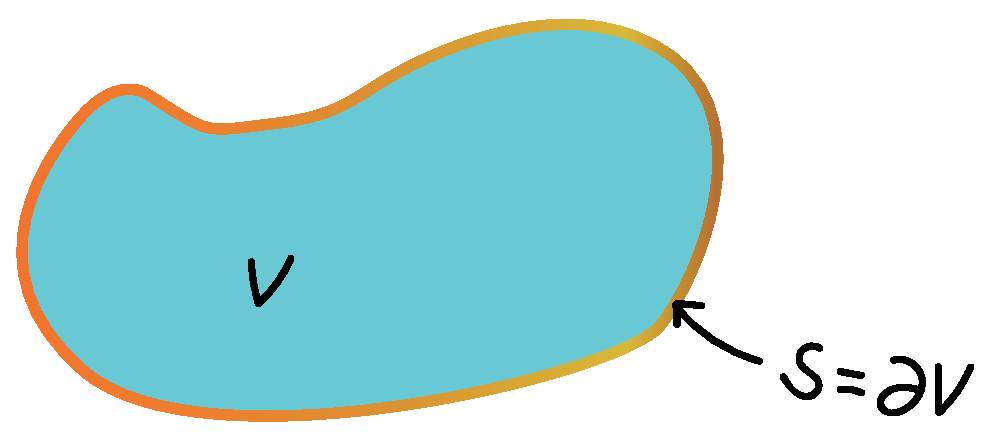
\includegraphics[width=\linewidth]{src/UniquenessTheoremI.eps}
		\caption{第一唯一性定理}
		\label{fig:第一唯一性定理}
	\end{subfigure}
	\begin{subfigure}{.3\textwidth}
		\centering
		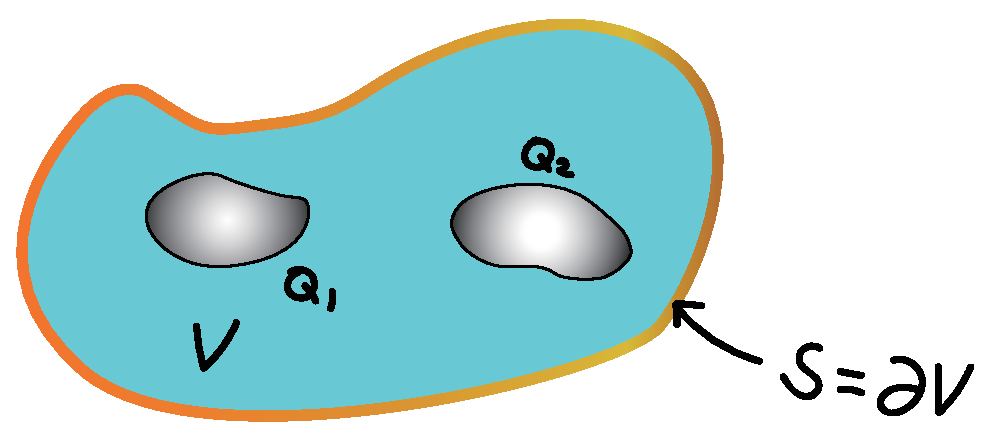
\includegraphics[width=\linewidth]{src/UniquenessTheoremII.eps}
		\caption{第二唯一性定理}
		\label{fig:第二唯一性定理}
	\end{subfigure}
	\caption{}
\end{figure}
\begin{finale}
	\begin{theorem}[第一唯一性定理]
		如\cref{fig:第一唯一性定理}, 若
		\begin{cenum}
			\item $S = \partial V$上的电势$\restr{\varphi}{S}$给定;
			\item $V$内部的电荷分布$\rho$已知;
		\end{cenum}
		则$\varphi$在$V$内唯一确定.
	\end{theorem}
	\begin{theorem}[第二唯一性定理]
		如\cref{fig:第二唯一性定理}, 若
		\begin{cenum}
			\item $S = \partial V$上的电势$\restr{\varphi}{S}$给定;
			\item 诸导体上电荷量$Q_i$给定;
			\item $V$内部的电荷分布$\rho$已知;
		\end{cenum}
		则$\varphi$在$V$内唯一确定.
	\end{theorem}
	\begin{corollary}[导体静电场叠加原理] 
		设空间中有固定导体,
		\begin{cenum}
			\item 当诸导体电势为$\varphi_i$, 相应带电量为$Q_i$, 空间电势为$\varphi$;
			\item 当诸导体电势为$\varphi'_i$, 相应带电量为$Q'_i$, 空间电势为$\varphi'$;
		\end{cenum}
		则诸导体电势为$\varphi_i+\varphi'_i$时, 相应带电量为$Q_i+Q'_i$, 空间电势为$\varphi+\varphi'$.
	\end{corollary}
\end{finale}

% subsection 唯一性定理 (end)

\subsection{电像法} % (fold)
\label{sub:电像法}

\begin{finale}
	\begin{theorem}[电像法的原则]
		\quad
		\begin{cenum}
			\item 源电荷位置即解的有效位置;
			\item 像电荷之和恰好等于该区域内电荷之和.
		\end{cenum}
	\end{theorem}
\end{finale}

%\begin{table}[ht]
%	\centering
	\begin{longtable}{|c|c|c|c|c|}
		\hline
		导体 & 源位置 & 源电荷 & 像位置 & 像电荷\\
		\hline
		接地平面 & 上方$+d$ & $+q$ & 下方$-d$ & $-q$\\
		\hline
		接地平面 & 上方$+d$ & $\vp$ & 下方$-d$ & $\vp$沿$z$反射\\
		\hline
		电介质 & & & 上方$+d$ & $\displaystyle \frac{\epsilon_0\pare{\epsilon_2-\epsilon_1}}{\epsilon_2\pare{\epsilon_1+\epsilon_2}}q$ \\
		下方$\epsilon_2$ & 下方$-d$ & $+q$ & 下方$-d$ & $\displaystyle q\mapsto \frac{\epsilon_0}{\epsilon_2} q$ \\
		上方$\epsilon_1$ & & & 下方$-d$ & $\displaystyle \frac{\epsilon_0\pare{\epsilon_2-\epsilon_1}}{\epsilon_2\pare{\epsilon_1+\epsilon_2}}q $ \\
		\hline
		\multicolumn{2}{|c}{\raisebox{-\totalheight}{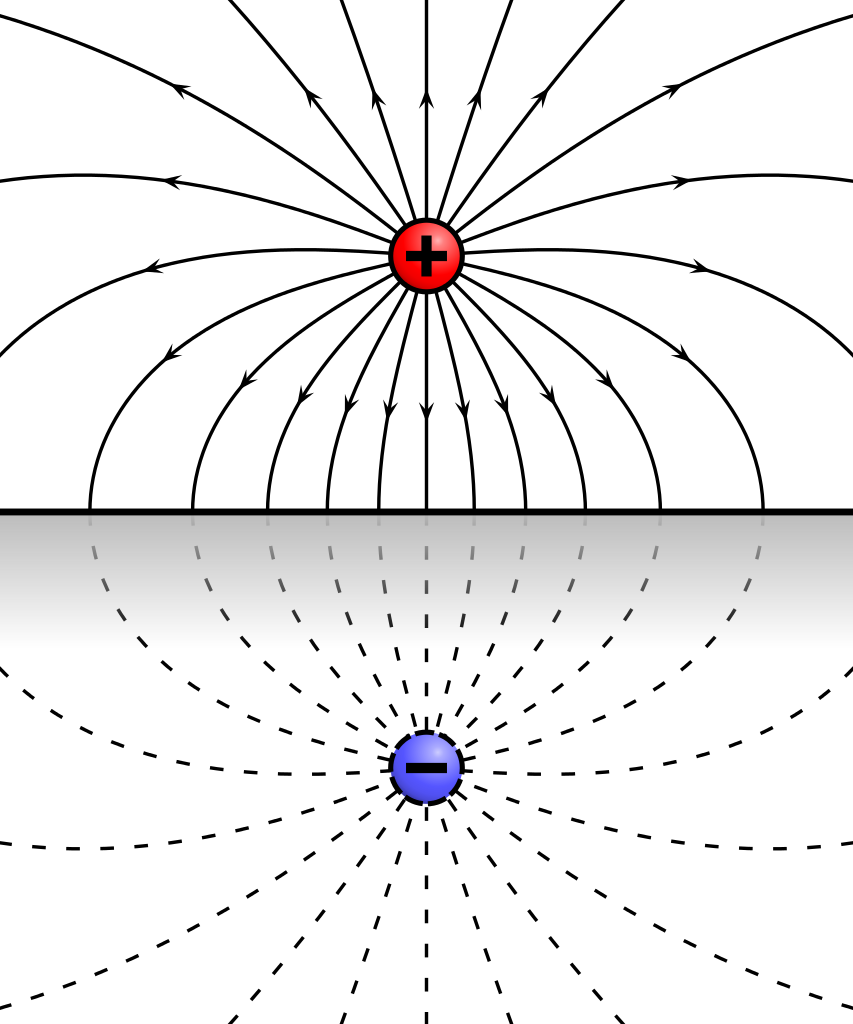
\includegraphics[height=4cm]{src/853px-VFPt_imagecharge_plane_horizontal_plusminus.eps}}} & \multicolumn{3}{c|}{\raisebox{-\totalheight}{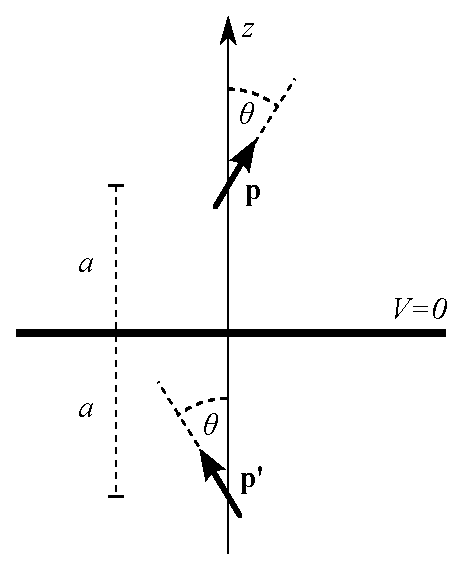
\includegraphics[height=4cm]{src/Image_of_dipole_in_plane.eps}}}\\
		\hline
		接地垂直 & 导体板间 & $+q$ & 连续$2$次反射 & $\pm q$\\
		\hline
		接地$60^\circ$ & 导体板间 & $+q$ & 连续$3$次反射 & $\pm q$ \\
		\hline
		\multicolumn{5}{|c|}{\raisebox{-\totalheight}{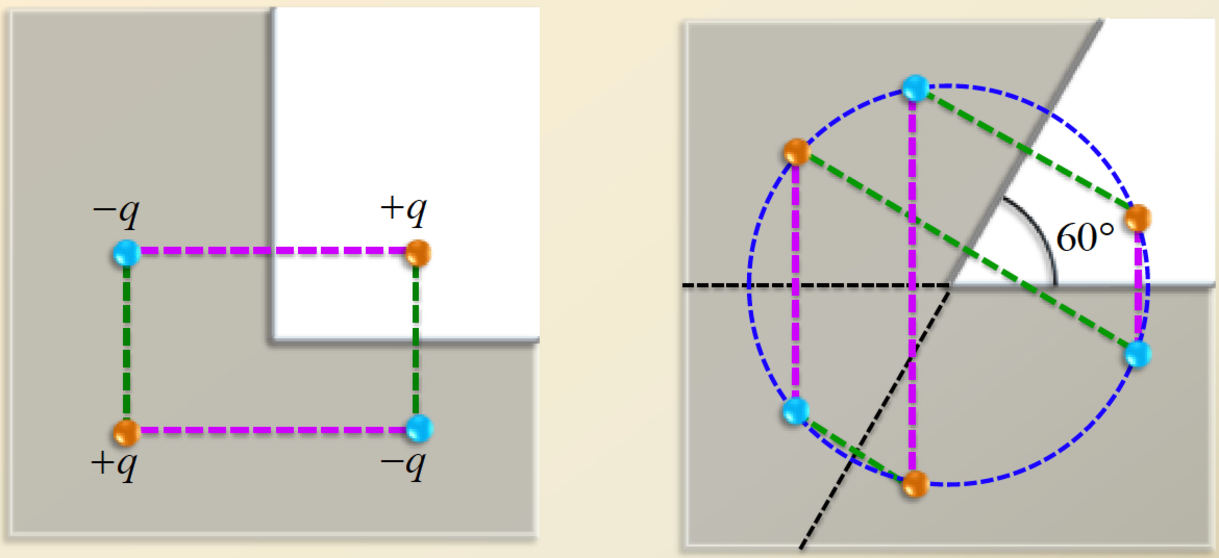
\includegraphics[height=4cm]{src/HexagonImageCharge.pdf}}}\\
		\hline
		接地球壳 & 球外$d$处 & $+q$ & 球内$\frac{R^2}{d}$处 & $-\frac{R}{d}q$\\
		\hline
		\multirow{2}{*}{带电球壳} & 球外$d$处 & $+q$ & 球内$\frac{R^2}{d}$处 & $q'=-\frac{a}{d}q$\\
		& 球壳 & $Q$ & 球内$O$处 & $Q-q'$\\
		\hline
		接地球壳 & 球内$d$处 & $+q$ &球外$\frac{R^2}{d}$处 & $-\frac{R}{d}q$\\
		\hline
		\multirow{2}{*}{恒$\varphi_0$球壳} & 球内$d$处 & $+q$ &球外$\frac{R^2}{d}$处 & $-\frac{R}{d}q$\\
		& 球壳表面 & 电势$\varphi_0$ & 球壳表面 & $\sigma' = \epsilon_0\varphi_0/R$\\
		\hline
		\multicolumn{5}{|c|}{\raisebox{-\totalheight}{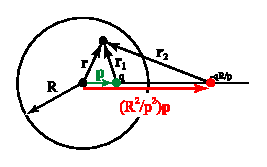
\includegraphics[height=4cm]{src/SphericalImage.eps}}}\\
		\hline
		接地球壳 & \multirow{2}{*}{轴上方$+d$} & \multirow{2}{*}{$+q$} & 轴上方$\frac{R^2}{d}$处 & $q'=-\frac{R}{d}q$\\
		组合平面 & & & 沿平面反射 & $\pm q,\pm q'$\\
		\hline
		接地球壳 & \multirow{2}{*}{板间球外$R$处} & \multirow{2}{*}{$+q$} & 板间球内$\frac{R^2}{d}$处 & $q'=-\frac{R}{d}q$\\
		组合垂直 & & & 连续$2$次反射 & $\pm q,\pm q'$\\
		\hline
		\multicolumn{5}{|c|}{\raisebox{-\totalheight}{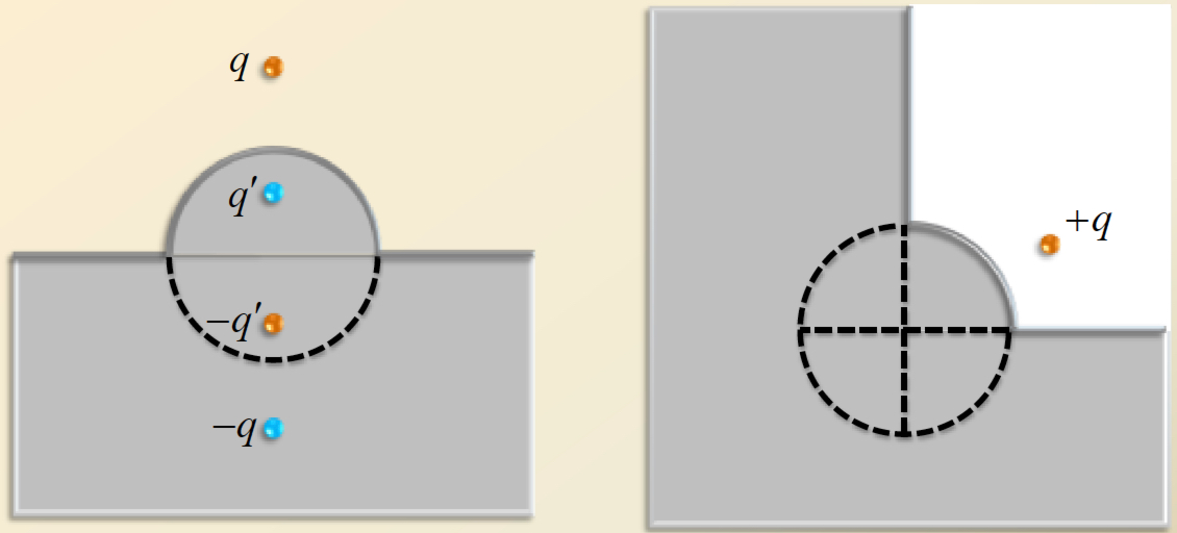
\includegraphics[height=4cm]{src/CombinationImage.pdf}}}\\
		\hline
		接地圆柱 & 柱外$d$处 & $+\lambda$ & 柱内$\frac{R^2}{d}$处 & $-\lambda$\\
		\hline
	\multicolumn{5}{|c|}{\raisebox{-\totalheight}{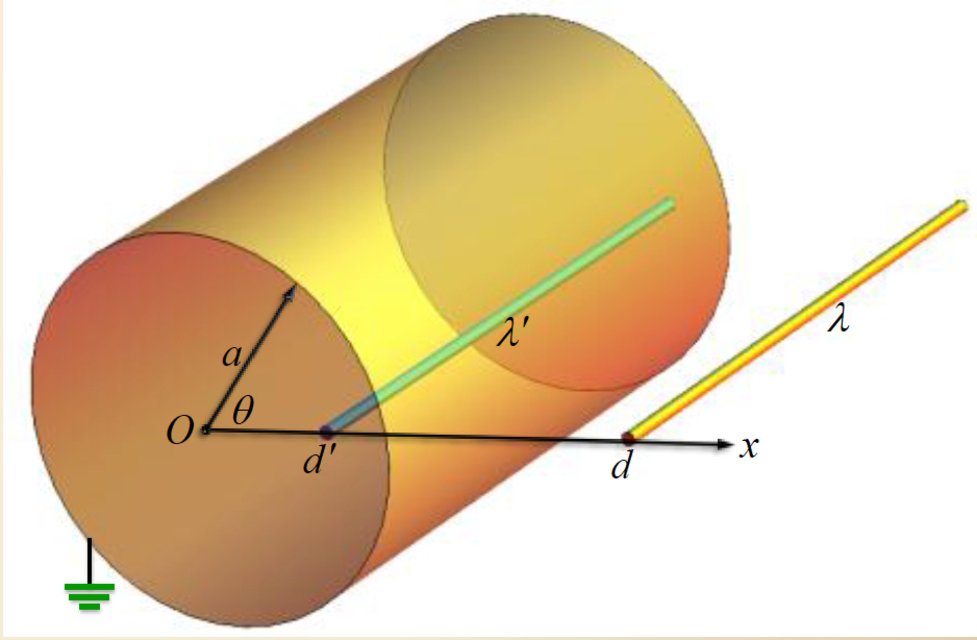
\includegraphics[height=4cm]{src/GroundedCylinder.pdf}}}\\
		\hline
	\end{longtable}
%\end{table}

\begin{pitfall}
	球壳的$q'\neq -q$, 但圆柱的$\lambda' = -\lambda$. 且二者的半径位置相同.
\end{pitfall}

\subsubsection{对称性论证} % (fold)
\label{ssub:对称性论证}

\begin{finale}
	对于具有旋转对称性的构型, 通过对线圈的$U$积分求出轴线上的$U$和$\vE$.
\end{finale}

% subsubsection 对称性论证 (end)

% subsection 电像法 (end)

\subsection{积分及其他数学} % (fold)
\label{sub:积分及其他数学}

常用积分:
\begin{align*}
	\int \sqrt{x^2+z^2} &= \half x\sqrt{x^2+z^2} + \half z^2 \ln\pare{x+\sqrt{x^2+z^2}}. \\
	\int \rec{\sqrt{x^2+z^2}}\,\rd{x} &= \ln \pare{x+\sqrt{x^2+z^2}}.\\
	\int \frac{x}{\sqrt{x^2+z^2}}\,\rd{x} &= \sqrt{x^2+z^2}.\\
	\int \rec{\pare{x^2+z^2}^{3/2}}\,\rd{x} &= \frac{x}{z^2\sqrt{x^2+z^2}}.\\
	\int \frac{x}{\pare{x^2+z^2}^{3/2}}\,\rd{x} &= -\rec{\sqrt{x^2+z^2}}.\\
	\int \frac{x^2}{\pare{x^2+z^2}^{3/2}}\,\rd{x} &= -\frac{x}{\sqrt{x^2+z^2}} + \ln\abs{x+\sqrt{x^2+z^2}}.\\
	\int \rec{\sqrt{r^2+z^2-2rzu}}\,\rd{u} &= \rec{rz}\sqrt{r^2+z^2-2rzu}. \\
	\int \frac{1}{1+t}\frac{1}{\sqrt{1+\pare{r^2+1}t}}\,\rd{x} &= \frac{2}{r}\arctan\frac{\sqrt{1+\pare{r^2+1}x}}{r}.\\
	\int \frac{1+r}{r^2}e^{-r}\,\rd{r} &= -\frac{e^{-r}}{r}.\\
	\int re^{-r}\,\rd{r} &= e^{-r}\pare{-1-r}.\\
	\int r^2e^{-r}\,\rd{r} &= e^{-r}\pare{-2-2r-r^2}.\\
	\int r^n e^{-r}\,\rd{r} &= e^{-r}\pare{-n! - \frac{n!}{1!} r - \frac{n!}{2!} r^2 - \cdots - \frac{n!}{n!}r^n}.
\end{align*}
\begin{pitfall}
	对于$y''=\lambda y^n$型的方程, 不能通过设$y=\pare{a x + b}^{\mu}$求解, 必须分离变量.
\end{pitfall}
Legendre多项式展开:
\begin{align*}
	\rec{\sqrt{1-2x\cos\theta+x^2}} &= \sum_{n=0}^\infty P_n\pare{\cos\theta}x^n. \\
	P_0\pare{x} &= 1,\\
	P_1\pare{x} &= x,\\
	P_2\pare{x} &= \half\pare{3x^2-1},\\
	P_3\pare{x} &= \half\pare{5x^3-3x^2}.
\end{align*}
曲线坐标系下的散度:
\begin{align*}
	\div\vF &= \rec{r^2}\ddelon{}{r}\pare{r^2F_r} + \rec{r\sin\theta} \ddelon{}{\theta}\pare{\sin\theta F_\theta} + \rec{r\sin\theta} \ddelon{F_\varphi}{\varphi}.\\
	\div\vF &= \rec{s}\ddelon{}{s}\pare{s F_s} + \rec{s}\ddelon{F_\varphi}{\varphi} + \ddelon{F_z}{z}.
\end{align*}

% subsection 积分及其他数学 (end)

\subsection{结论} % (fold)
\label{sub:结论}

\subsubsection{一般静电学} % (fold)
\label{ssub:一般静电学}

\begin{finale}
	cf.G.2.43., 计算电荷分布之一部受令一部施加的力时, 可直接对$\rho \vE$积分, 盖任何分布皆不对自身有静电力. 
\end{finale}
\begin{finale}
	cf.G.2.33., 将小量$\rd{q}$沿等势面涂抹, 做功为零.
\end{finale}
\begin{pitfall}
	cf.M.3.14., 计算电荷分布能量时, 若为外场导致能量则无需$\half$因子, 反之自能需要$\half$因子.
\end{pitfall}
\begin{finale}
	电荷分布能量为
	\[ W = \sum_i W_{i\,\text{self}} + \sum_{i\neq j} W_{ij\,\text{inter}}. \]
\end{finale}

% subsubsection 一般静电学 (end)

\subsubsection{电介质中的静电学} % (fold)
\label{ssub:电介质中的静电学}

\begin{finale}
	参考HG.2.21., 电介质中叠加原理亦适用, 适用电像法时可以先引入一个源电荷, 再引入第二个源电荷.
\end{finale}
\begin{finale}
	\begin{cenum}
		\item 电介质填充介面为等势面时, $\vD$前后不变, 即$\vE \mapsto \vE/\epsilon_r$.
		\item 电介质填充介面沿电场线时, 可假设$\vE \mapsto \alpha \vE$处处一致成立, 通过适当边界条件确定$\alpha$. 参考M.2.3.31.
	\end{cenum}
\end{finale}
\begin{finale}
	介质自动将任何自由电荷约化为$q\mapsto q/\epsilon_r$(例如介质内嵌电荷), $\sigma\mapsto \sigma/\epsilon_r$(例如电容边界处).
\end{finale}

% subsubsection 电介质中的静电学 (end)

\subsubsection{电容器相关} % (fold)
\label{ssub:电容器相关}

\begin{finale}
	电容器几何量
	\[ U = \frac{Q}{C}, \quad Q = CU, \quad C = \frac{Q}{U}. \]
	\[ W = \half \frac{Q^2}{C} = \half CU^2 = \half QU. \]
\end{finale}
\begin{finale}
	电容器串联时, 能量$W_1\propto C_2$, $W_2\propto C_1$, 并联时$W_1\propto C_1$, $W_2\propto C_2$, 注意与电阻的情形区分.
\end{finale}
\begin{finale}
	参考M.3.34., 3.35., 3.47, 带电电容器的串接: 电容直接视为并联, 电量直接中和. 电容器内不完全插入电介质, 分解为电容器的串/并联.
\end{finale}
\begin{finale}
	参考M.2.3.4., 2.3.5., 2.3.6., 2.3.25., 存在共用极板/覆叠极板时, 考虑将极板拆分为电容并联.
\end{finale}
\begin{finale}
	参考M.3.38., 3.39., 电容器极板受力
	\[ F = \half \epsilon E^2 S. \]
	区别于真空下的受力(cf.G.2.37.)
	\[ F = \half \epsilon_0 E^2 S. \]
\end{finale}
\begin{finale}
	参考M.3.40., 电容器对导体的力矩为
	\[ M = \pare{\ddelon{W}{\theta}}_U = -\pare{\ddelon{W}{\theta}}_Q. \]
	$M$为正时力矩使$\theta$有增大趋势.
\end{finale}
\begin{finale}
	通过对$F$积分计算电容吸入电介质做功时, 自电介质达边界处始积分.
\end{finale}

% subsubsection 电容器相关 (end)

\subsubsection{电流} % (fold)
\label{ssub:电流}

\begin{finale}
	\[ \sigma = \frac{ne^2\tau}{m}. \]
\end{finale}
\begin{finale}
	两个理想导体在无限均匀电介质中成立
	\[ RC = \rho\epsilon. \]
\end{finale}
\begin{finale}
	体电流发热功率
	\[ P = \iint \sigma E^2\,\rd{V}. \]
\end{finale}
\begin{pitfall}
	\[ R = \int_a^b \frac{\rd{r}}{\sigma \cdot S}. \]
	特别地, 对于球壳,
	\[ R = \int_a^b \frac{\rd{r}}{\sigma \cdot 4\pi r^2}. \]
	尤其注意分子分母的位置.
\end{pitfall}

% subsubsection 电流 (end)

% subsection 结论 (end)

% section 特殊构型_唯一性定理_电像法与green定理等 (end)

% 该文档作为转换器的实例
% 中文悉数被转化为英文代码, 生成html后再转化回来
% 相同的中文应被转化为相同的代码, 以保证label的正常工作


% 宏实现: longtable环境一律直接转化为tabular环境, 否则无法正常显示横线
% 宏实现: subfigure一律直接转化为figure, 否则无法正常加载. figure是可以嵌套的
% 宏实现: pitfall与finale一律转化为\HCode{<div>}*\HCode{</div>}环绕, 手动设定样式表


% 代码规范: tikz图必须单独编译
% 代码规范: 任何情况下公式内不应当出现中文

\end{document}
